\subsection{Controllers}

		În afară de separarea conceptuală a arhitecturii MVC, Laravel se folosește și de un sistem de gestionare a rutelor aplicației. \cite{laravel_controllers}

		Spre deosebire de alte librării precum CakePHP, Laravel nu pune mult accent pe numele Controller-ului.
		Ci mai degrabă se folosește de un fișier principal unde se specifică legătura dintre un URL și un Controller, ce se regăsește în cadrul proiectului Laravel la:
		\begin{verbatim}
			/routes/web.php
		\end{verbatim}

		În cazul proiectului de gestionare a cererilor de despăgubire, se pune foarte mult accent pe securitatea datelor.
		Din acest motiv, printre primele linii ale fișierului, regăsim
		\begin{verbatim}
		URL::forceSchema("https");
		\end{verbatim}
		ce indică schemei de rutare Laravel rescrierea oricărui link a folosi HTTPS, pentru a menține legătura encriptată cu clientul.
		În cazul în care clientul cere varianta normală (HTTP) a unei pagini, el este redirectat automat spre varianta HTTPS.
		Din acest motiv nu am activat în cadrul „CloudFlare” opțiunea de „Automatic HTTPS rewrites” (rescrieri automate HTTPS), pentru că deja se ocupă de asta librăria Laravel.
		În cazul în care aș fi activat opțiunea respectivă, s-ar fi bătut cap în cap cu implementarea Laravel.
		Nu am descoperit cauza, dar încă investighez.

		Un mare avantaj al sistemului de rutare este gruparea rutelor prin includerea automată a unor „middleware”, precum sistemul de asigurare a unui utilizator cu o sesiune activă, dar și scurtarea căilor Controller-lor sau căilor. Se poate observa prin intermediul codului:
\begin{Verbatim}
Route::group([
	'middleware' => 'auth',
	'prefix' => 'admin',
	'namespace' => 'Admin',
], function () {
	// funcții aici
});
\end{Verbatim}

	\label{alg:group}

	\begin{itemize}
		\item prefixarea căilor cu „admin”
		\item în numele spațiului claselor „Admin”
		\item ce sigur va conține „middleware”-ul „auth”
	\end{itemize}

	Laravel în afară de cererile simple poate combina mai multe dintre cererile simple într-o „resursă”.
	Cererile simple pot fi:
	\begin{itemize}
		\item GET - citește una sau mai multe informații.
		\item POST - salvează (de obicei prin adăugare) o informație (de obicei nouă).
		\item PUT / PATCH - modifică de obicei o informație deja existentă.
		\item DELETE - șterge informația.
	\end{itemize}

	O „resursă” în Laravel atribuie rutele „CRUD” (Create / Read / Update / Delete) unui Controller cu o singură linie de cod:
	\begin{verbatim}
		Route::resource('obiecte', 'ObiectController');
	\end{verbatim}
	Și mulțumită consolei Artisan, se poate construi la fel de rapid și codul necesar unui astfel de Controller, prin simpla comandă:
	\begin{verbatim}
		php artisan make:controller ObiectController --resource
	\end{verbatim}

	Următoarele acțiuni sunt definite și gata de a fi modificate de dezvoltator pentru a fi gestionate:
	\begin{center}
	\begin{tabular}{ | l | l | l | l |}
	\hline
	Verb & URI & Acțiune & Nume rută \\
	\hline
	GET & \verb|/obiecte| & index & obiecte.index \\
	GET & \verb|/obiecte/create| & create & obiecte.create \\
	POST & \verb|/obiecte| & store & obiecte.store \\
	GET & \verb|/obiecte/{obiect}| & show & obiecte.show \\
	GET & 	\verb|/obiecte/{obiect}/edit| & edit & obiecte.edit \\
	PUT/PATCH & \verb|/obiecte/{obiect}| & update & obiecte.update \\
	DELETE & \verb|/obiecte/{obiect}| & destroy & obiecte.destroy \\
	\hline
	\end{tabular}
	\end{center}

	În cadrul proiectului, am următoarea structură a directoarelor controalelor:

	\begin{itemize}
		\item Folderul implicit:
			\begin{itemize}
				\item \verb|MessagesController.php| - gestionează mesajele trimise între client și operatorul cererii de despăgubire.
				\item \verb|HelperController.php| - ajută la testarea sistemului de mail și menținerea sesiunii clientului.
				\item \verb|ClaimsController.php| - construiește cererea de despăgubire, afișează pagina principală și clauza de confidențialitate.
			\end{itemize}
		\item Folderul \verb|Json|:
			\begin{itemize}
				\item \verb|ImagesController.php| - gestionează încărcarea pozelor asincron de către client sau operator spre soluția distribuită de stocare a datelor --- Amazon Web Services S3.
			\end{itemize}
		\item Folderul \verb|Admin|:
			\begin{itemize}
				\item Folderul \verb|Json|:
				\begin{itemize}
					\item \verb|SearchController.php| - gestionează încărcarea rezultatelor parțiale asincron de către operator.
				\end{itemize}
				\item
					\verb|ClaimsController.php| - gestionează vizualizarea, modificarea și finalizarea cererilor de despăgubire.
					În cazul în care se găsește în parametrul GET (ce urmează dupa „?” în cadrul URL-ului) \verb|id|, se va încerca redirecționarea spre cererea de despăgubire cu acel \verb|id|.
					Dacă este aplicată o căutare, afișează toate rezultatele, altfel paginează câte 100 cereri pe pagină folosind Eloquent.

					În momentul în care se salvează o cerere noua de despăgubire, se trimite un mail cu datele create către căsuța principală a operatorilor sistemului și către client.
					El este rugat să-și verifice și căsuța de mail, iar cât mai curând să încarce toate pozele necesare completării dosarului său.

					Sistemul de căutare poate căuta în:
					\begin{itemize}
						\item Număr de telefon.
						\item Nume.
						\item Prenume.
						\item Model telefon.
						\item Email.
						\item O dată de început a facturii.
						\item O dată de sfârșit a facturii.
					\end{itemize}
				\item \verb|DecisionController.php| - gestionează vizualizarea, modificarea și posibila șterge a deciziilor cererilor de despăgubire.
				În cazul în care există o căutare, acesta caută și în cerere, și în decizie, folosind următoarele câmpuri:
				\begin{itemize}
						\item Număr de telefon.
						\item Nume.
						\item Prenume.
						\item Model telefon.
						\item Email.
						\item O dată de început a înregistrării cererii.
						\item O dată de sfârșit a înregistrării cererii.
						\item Numele produsului conform deciziei.
				\end{itemize}

				În cazul creării unei noi decizii în funcție de o cerere de despăgubire, se încearcă mai întâi găsirea automată a vânzării asociate după numărul facturii.
				Dacă căutarea nu reușește, atunci se va indica utilizatorului necesitatea unei construirii unei legături manuale.

				Pentru a salva o legătură între o cerere de despăgubire și o decizie, trebuie să existe următoarele câmpuri completate valid, ce nu trebuie să fie vide:
				\begin{itemize}
					\item \verb|claim_id| - id-ul cererii de despăgubire.
					\item \verb|product_name| - numele produsului de pe factură.
					\item \verb|product_price| - prețul produsului de pe factură.
					\item \verb|product_premium_price| - prețul asigurării.
					\item \verb|product_sale_date| - data vânzării produsului.
					\item \verb|product_expire_date| - data expirării asigurării.
				\end{itemize}

				Dacă se salvează cu succes decizia, ea va apărea asincron, integrată în pagina de vizualizării a cererii de despăgubire, în josul paginii.
				\item \verb|HomeController.php| - gestionează o interfață simplă cu două rapoarte, împreună datele de contact personale, în cazul în care apare vreo problemă.

				Sistemul arată precum în figura~\ref{fig:home_page}.

				\begin{figure}
					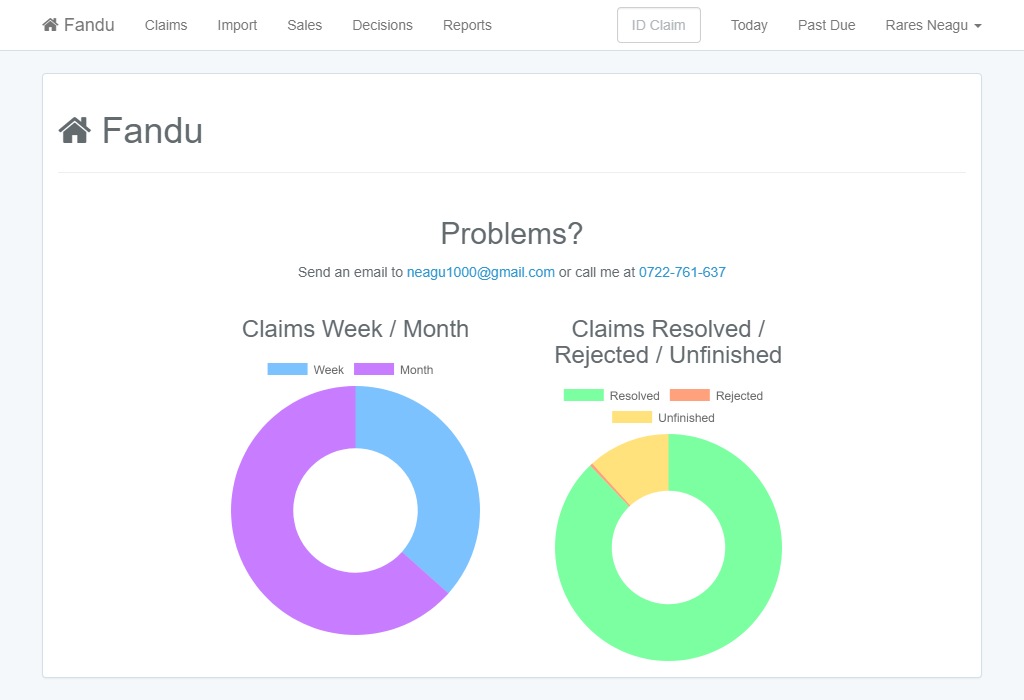
\includegraphics[width=\linewidth]{../imagini/home_page.png}
					\caption{Pagina acasă}
					\label{fig:home_page}
				\end{figure}

				\item \verb|ImportController.php| - gestionează sistemul de introducere de date prin fișierele Excel în sistem.

				Acesta construiește automat un adaptor ce preia fișierul Excel și afișează un răspuns, de obicei printr-un View.
				Este împărțit în două categorii de fișiere --- cele standarde, despre care s-au discutat la momentul definitivării modulelor și cele personalizate pentru fișierele apărute pe parcursul dezvoltării.

				Această diferențiere apare mulțumită notificării trimise pe email în momentul salvării cu succes a datelor din fișierele standard.

				Sistemul arată precum în figura~\ref{fig:imports}.

				\begin{figure}
					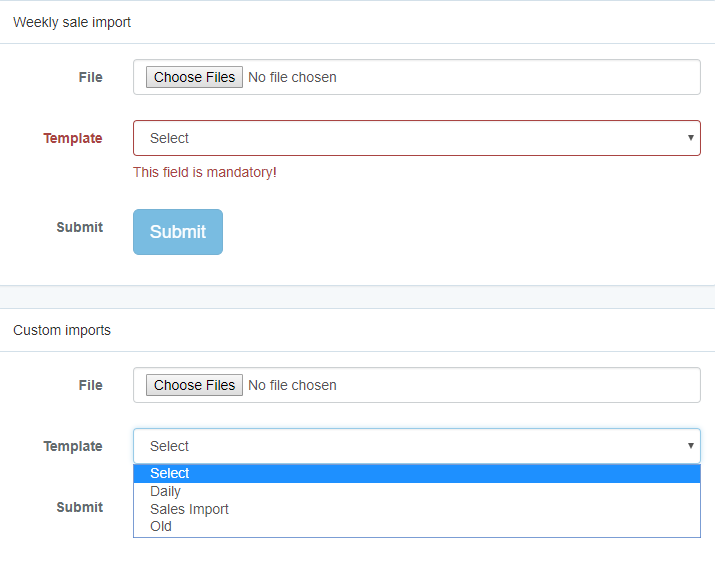
\includegraphics[width=\linewidth]{../imagini/imports.png}
					\caption{Sistemul de introducere a datelor}
					\label{fig:imports}
				\end{figure}

				\item \verb|ReportsController.php| - gestionează sistemul de rapoarte.
				Inițial scris astfel încât dintr-o singură metodă să reiasă un raport, acum funcționează modular și necesită cod asincron JavaScript pentru a scoate un raport.

				Sistemul a fost conceput astfel din cauza numărului imens de date ce trebuia să treacă prin modulul ce transformă datele în fișierul de format Excel.
				Fiecare raport are o metodă ce decide dacă mai are nevoie de pași suplimentari și deci de încă o cerere asincronă, pentru a folosi apoi la final, la pasul de combinare, toate datele din fișiere pentru a scoate raportul în formatul dorit.
				Avantajul folosirii fișierelor temporare și a mai multor apeluri asincrone este de a face interfața cu utilizatorul mai plăcută și în același timp de a reduce din consumul de memorie.

				Pentru a arăta interactiv că fișierul s-a descărcat cu succes, setez un „cookie” atunci când descarcă fișierul utilizatorul, iar în pagina de rapoarte aștept apariția acestui „cookie” pentru a semnala finalizarea descărcării.
				După ce l-am identificat, îl șterg setându-l să expire pe „1 Ianuarie 1970 00:00:01 GMT”.

				Sistemul arată precum în figura~\ref{fig:reports}.

				\begin{figure}
					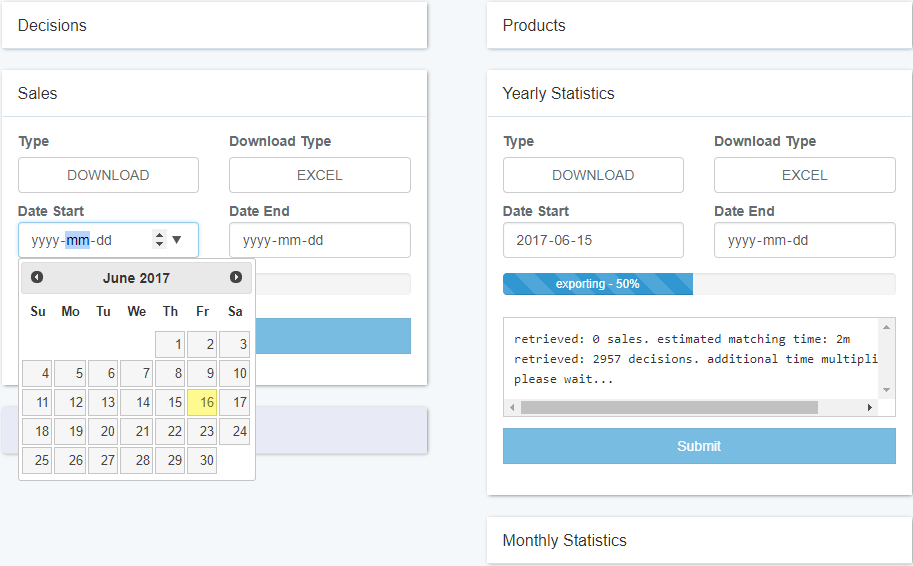
\includegraphics[width=\linewidth]{../imagini/reports.png}
					\caption{Sistemul de rapoarte}
					\label{fig:reports}
				\end{figure}

				\item \verb|SalesController.php| - gestionează existența, modificarea, afișarea și căutarea vânzărilor introduse în sistem.

				Funcția de căutare, prezentă în figura~\ref{fig:sales_search} se referă la:
				\begin{itemize}
					\item \verb|Product| - Numele produsului căutat.
					\item \verb|Customer| - Numele clientului ce a cumpărat produsul.
					\item \verb|Date Start| - Data de început de când s-ar fi putut vinde produsul.
					\item \verb|Date End| - Data de sfârșit de când s-ar fi putut vinde produsul.
					\item \verb|Date Added| - Data când a fost importat fișierul (acest câmp, conform statisticilor Google Analytics, este degeaba și va fi scos într-o variantă ulterioară, cel mai probabil).
					\item \verb|External ID| - Numărul facturii.
				\end{itemize}
				\begin{figure}
					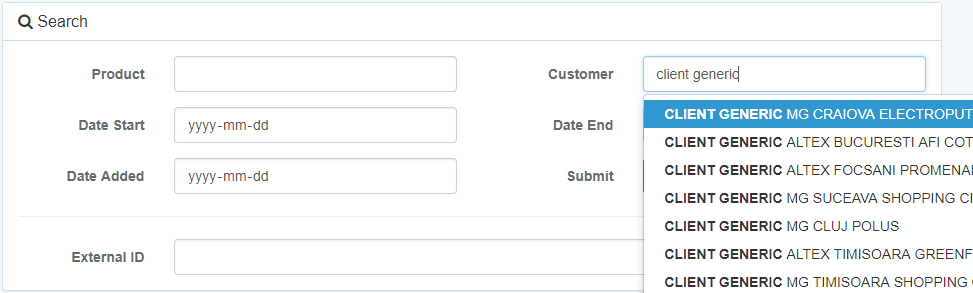
\includegraphics[width=\linewidth]{../imagini/sales_search.png}
					\caption{Căutarea vânzărilor}
					\label{fig:sales_search}
				\end{figure}
				\item \verb|ProductsController.php| și \verb|AssurancesController.php| - gestionează doar construirea și ștergea
					produselor, respectiv asigurărilor, din interfața ce modifică vânzările.
					Nu au niciun alt rol.
				\item \verb|ExportController.php| - gestionează compunerea unor fișiere .CSV cu toate datele, fără a fi trecute printr-un filtru, a unui tabel din baza de date.

				A fost folosit într-un moment de „criză”, unde era nevoie obligatoriu de a putea scoate datele din sistemul informatic pentru a trimite un raport rapid, când nu era gata sistemul de raportare.

				Nu are interfață grafică.

				\item \verb|BackupController.php| - gestionează sistemul actual de salvare a bazei de date de orice operator al companiei.
				Acest sistem necesită din cauza acelorași probleme de memorie mai multe apeluri, pentru a construi arhiva cu toate datele tabelelor bazei de date.
				Se folosește de punctul de colectare:
				\begin{verbatim}
				storage_path("app/*.sql")
				\end{verbatim}
				și comprimă tot ce găsește obținut din apelurile asincrone din JavaScript anterioare pentru a compune o arhiva finală „.tar.gz”.

				Pe serverul de producție este foarte lentă compunerea arhivei finale, așa că voi considera scoaterea comprimării arhivei și transmiterea folosind unei arhive „.zip”.
				Nu pot să folosesc și algoritmi de comprimare a datelor pentru arhivele „.zip” deoarece s-a adăugat abia în PHP 7 opțiunea.

				În prima parte a figurii~\ref{fig:backups} este interfața ce permite salvarea individuală a tabelelor.
				În momentul apăsării butonului de „Download All”, o să arate precum în a doua parte a figurii.

				\begin{figure}
					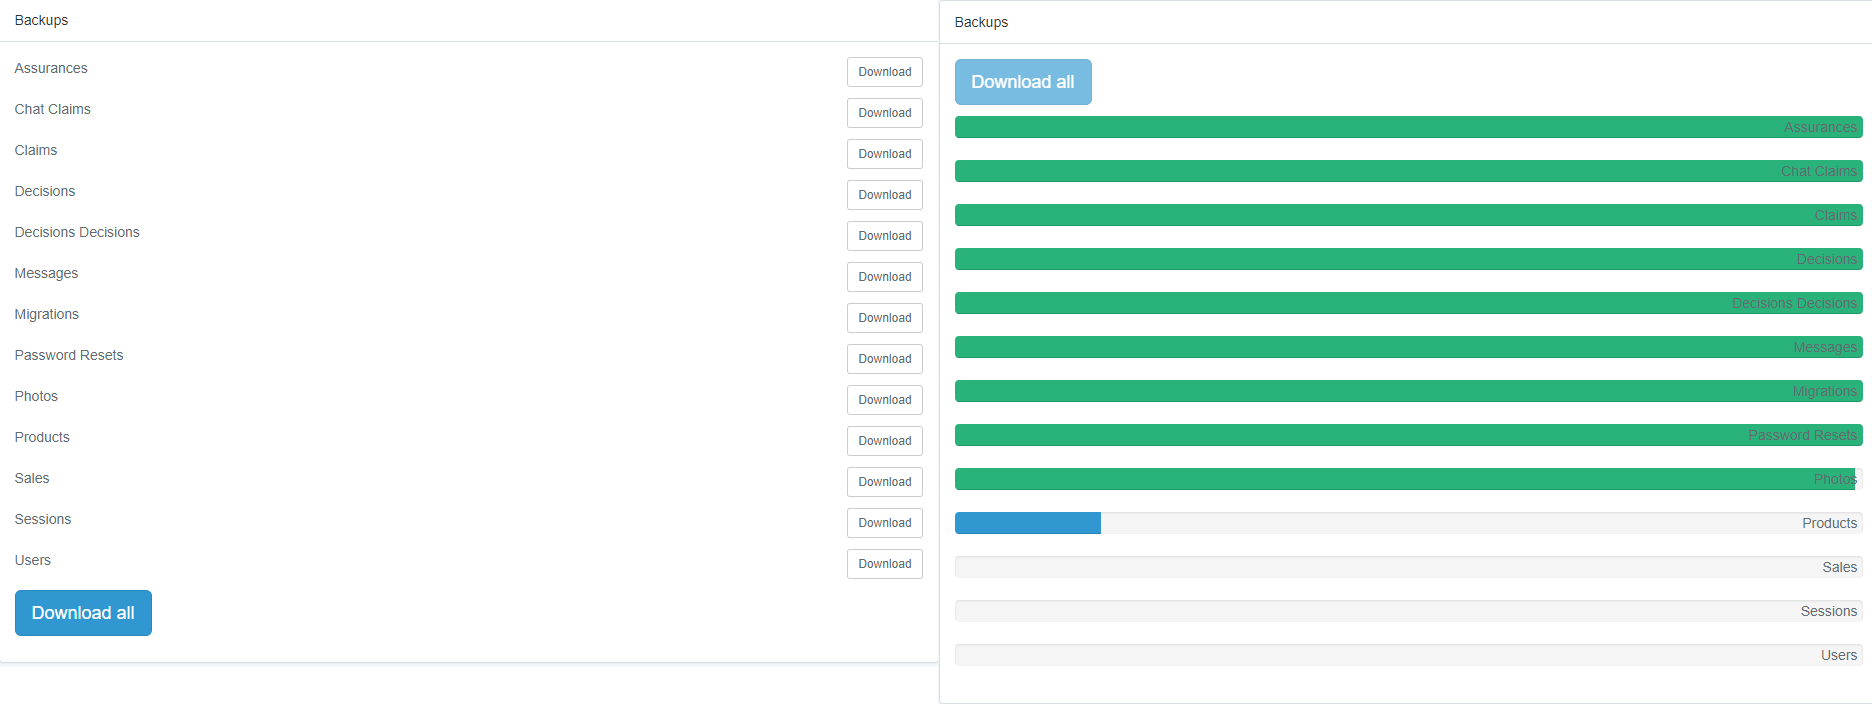
\includegraphics[width=\linewidth]{../imagini/backups.png}
					\caption{Sistemul de salvare a bazei de date}
					\label{fig:backups}
				\end{figure}


				\item \verb|SettingsController.php| - gestionează
			\end{itemize}
			\item Folderul \verb|Auth| este cel construit implicit de Laravel atunci când construiește codul de a autentifica utilizatorii.

			O mică modificare ce s-ar putea să treacă neobservată este schimbarea controller-ului \verb|RegisterController| de a fi folosit împreună cu grupul algoritmului~\ref{alg:group}, ceea ce indică puterea de a adăuga utilizatori aparține doar utilizatorilor de sistem.

			De asemenea, singurul mod prin care se poate înregistra un utilizator nou este prin cunoașterea adresei specifice Controller-ului:
			\begin{Verbatim}
Route::get('register', [
	'middleware' => 'auth',
	'as' => 'register',
	'uses' => 'Auth\RegisterController@showRegistrationForm
']);
Route::post('register', [
	'middleware' => 'auth',
	'as' => 'register.post',
	'uses' => 'Auth\RegisterController@register'
]);
			\end{Verbatim}


			Pentru a nu fi blocați pe dinafară, se adaugă mereu un utilizator în baza de date printr-o migrare.
	\end{itemize}
